

\tikzset{every picture/.style={line width=0.75pt}} %set default line width to 0.75pt        

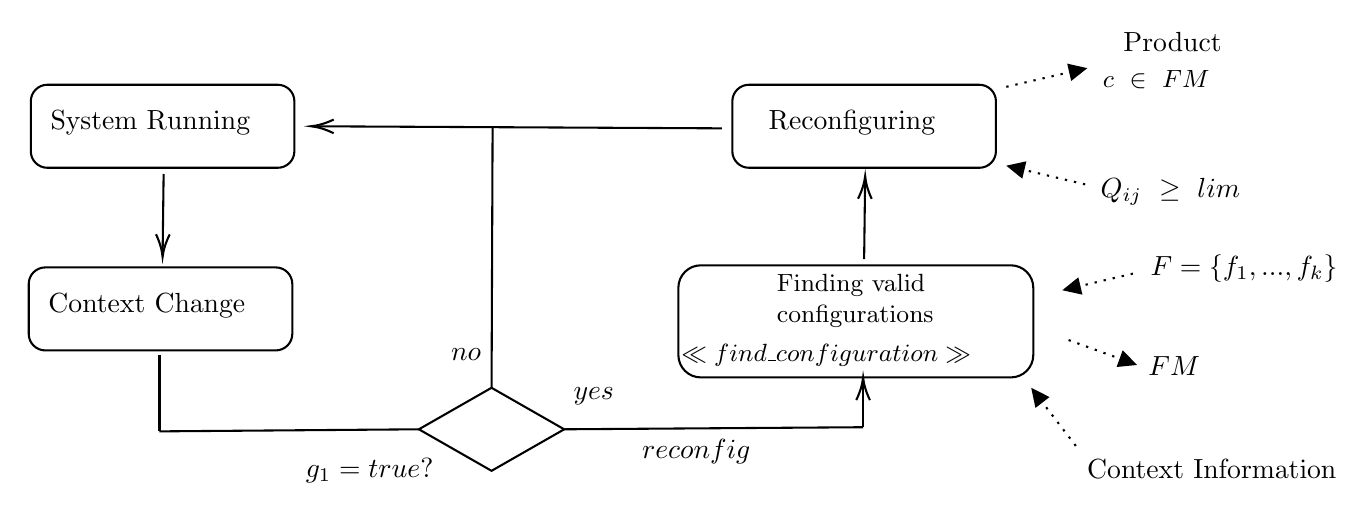
\begin{tikzpicture}[x=0.75pt,y=0.75pt,yscale=-1,xscale=1]
%uncomment if require: \path (0,244); %set diagram left start at 0, and has height of 244

%Rounded Rect [id:dp8066480632996035] 
\draw   (9,40) .. controls (9,35.58) and (12.58,32) .. (17,32) -- (128,32) .. controls (132.42,32) and (136,35.58) .. (136,40) -- (136,64) .. controls (136,68.42) and (132.42,72) .. (128,72) -- (17,72) .. controls (12.58,72) and (9,68.42) .. (9,64) -- cycle ;
%Rounded Rect [id:dp09986312472167136] 
\draw   (8,128) .. controls (8,123.58) and (11.58,120) .. (16,120) -- (127,120) .. controls (131.42,120) and (135,123.58) .. (135,128) -- (135,152) .. controls (135,156.42) and (131.42,160) .. (127,160) -- (16,160) .. controls (11.58,160) and (8,156.42) .. (8,152) -- cycle ;
%Rounded Rect [id:dp3203334247066908] 
\draw   (321,129.8) .. controls (321,123.84) and (325.84,119) .. (331.8,119) -- (481.2,119) .. controls (487.16,119) and (492,123.84) .. (492,129.8) -- (492,162.2) .. controls (492,168.16) and (487.16,173) .. (481.2,173) -- (331.8,173) .. controls (325.84,173) and (321,168.16) .. (321,162.2) -- cycle ;
%Straight Lines [id:da7215475210798592] 
\draw    (342,53) -- (146,52.01) ;
\draw [shift={(144,52)}, rotate = 0.29] [color={rgb, 255:red, 0; green, 0; blue, 0 }  ][line width=0.75]    (10.93,-3.29) .. controls (6.95,-1.4) and (3.31,-0.3) .. (0,0) .. controls (3.31,0.3) and (6.95,1.4) .. (10.93,3.29)   ;
%Straight Lines [id:da566488552820097] 
\draw    (73,75) -- (72.52,113) ;
\draw [shift={(72.5,115)}, rotate = 270.72] [color={rgb, 255:red, 0; green, 0; blue, 0 }  ][line width=0.75]    (10.93,-3.29) .. controls (6.95,-1.4) and (3.31,-0.3) .. (0,0) .. controls (3.31,0.3) and (6.95,1.4) .. (10.93,3.29)   ;
%Straight Lines [id:da03600720187770856] 
\draw  [dash pattern={on 0.84pt off 2.51pt}]  (509,155) -- (539.18,165.97) ;
\draw [shift={(542,167)}, rotate = 199.98] [fill={rgb, 255:red, 0; green, 0; blue, 0 }  ][line width=0.08]  [draw opacity=0] (8.93,-4.29) -- (0,0) -- (8.93,4.29) -- cycle    ;
%Rounded Rect [id:dp7101206593267378] 
\draw   (347,40) .. controls (347,35.58) and (350.58,32) .. (355,32) -- (466,32) .. controls (470.42,32) and (474,35.58) .. (474,40) -- (474,64) .. controls (474,68.42) and (470.42,72) .. (466,72) -- (355,72) .. controls (350.58,72) and (347,68.42) .. (347,64) -- cycle ;
%Straight Lines [id:da7286524767507477] 
\draw    (266,198) -- (410,197) ;
%Straight Lines [id:da695602580560019] 
\draw    (71,162) -- (71,199) ;
%Straight Lines [id:da47123812289807143] 
\draw    (410,175) -- (410,197) ;
\draw [shift={(410,173)}, rotate = 90] [color={rgb, 255:red, 0; green, 0; blue, 0 }  ][line width=0.75]    (10.93,-3.29) .. controls (6.95,-1.4) and (3.31,-0.3) .. (0,0) .. controls (3.31,0.3) and (6.95,1.4) .. (10.93,3.29)   ;
%Straight Lines [id:da7842612276994353] 
\draw  [dash pattern={on 0.84pt off 2.51pt}]  (517,80) -- (481.92,71.69) ;
\draw [shift={(479,71)}, rotate = 13.32] [fill={rgb, 255:red, 0; green, 0; blue, 0 }  ][line width=0.08]  [draw opacity=0] (8.93,-4.29) -- (0,0) -- (8.93,4.29) -- cycle    ;
%Straight Lines [id:da6842594623348534] 
\draw  [dash pattern={on 0.84pt off 2.51pt}]  (479,33) -- (515.08,24.67) ;
\draw [shift={(518,24)}, rotate = 167.01] [fill={rgb, 255:red, 0; green, 0; blue, 0 }  ][line width=0.08]  [draw opacity=0] (8.93,-4.29) -- (0,0) -- (8.93,4.29) -- cycle    ;
%Straight Lines [id:da2973367810568732] 
\draw    (410.98,78) -- (410.5,116) ;
\draw [shift={(411,76)}, rotate = 90.72] [color={rgb, 255:red, 0; green, 0; blue, 0 }  ][line width=0.75]    (10.93,-3.29) .. controls (6.95,-1.4) and (3.31,-0.3) .. (0,0) .. controls (3.31,0.3) and (6.95,1.4) .. (10.93,3.29)   ;
%Straight Lines [id:da9420001435559124] 
\draw  [dash pattern={on 0.84pt off 2.51pt}]  (540,123) -- (508.92,130.31) ;
\draw [shift={(506,131)}, rotate = 346.76] [fill={rgb, 255:red, 0; green, 0; blue, 0 }  ][line width=0.08]  [draw opacity=0] (8.93,-4.29) -- (0,0) -- (8.93,4.29) -- cycle    ;
%Flowchart: Decision [id:dp759598130534352] 
\draw   (231,178) -- (266,198) -- (231,218) -- (196,198) -- cycle ;
%Straight Lines [id:da367734053399414] 
\draw    (71,199) -- (196,198) ;
%Straight Lines [id:da5755851308332511] 
\draw    (231.5,52) -- (231,178) ;
%Straight Lines [id:da3242394337958049] 
\draw  [dash pattern={on 0.84pt off 2.51pt}]  (512.5,206) -- (492.83,180.38) ;
\draw [shift={(491,178)}, rotate = 52.48] [fill={rgb, 255:red, 0; green, 0; blue, 0 }  ][line width=0.08]  [draw opacity=0] (8.93,-4.29) -- (0,0) -- (8.93,4.29) -- cycle    ;

% Text Node
\draw (17,43) node [anchor=north west][inner sep=0.75pt]   [align=left] {System Running};
% Text Node
\draw (16,131) node [anchor=north west][inner sep=0.75pt]   [align=left] {Context Change};
% Text Node
\draw (367,122) node [anchor=north west][inner sep=0.75pt]  [font=\small] [align=left] {Finding valid\\configurations};
% Text Node
\draw (321,155.4) node [anchor=north west][inner sep=0.75pt]  [font=\small]  {$\ll find\_configuration\gg $};
% Text Node
\draw (546,161.4) node [anchor=north west][inner sep=0.75pt]    {$\llbracket FM\rrbracket $};
% Text Node
\draw (363,43) node [anchor=north west][inner sep=0.75pt]   [align=left] {Reconfiguring};
% Text Node
\draw (523,75.4) node [anchor=north west][inner sep=0.75pt]    {$Q_{ij} \ \geq \ lim$};
% Text Node
\draw (302,201.4) node [anchor=north west][inner sep=0.75pt]    {$reconfig$};
% Text Node
\draw (529,5) node [anchor=north west][inner sep=0.75pt]   [align=left] {\begin{minipage}[lt]{42.88pt}\setlength\topsep{0pt}
\begin{center}
Product
\end{center}

\end{minipage}};
% Text Node
\draw (547,112.4) node [anchor=north west][inner sep=0.75pt]    {$F=\{f_{1} ,...,f_{k}\}$};
% Text Node
\draw (524,23.4) node [anchor=north west][inner sep=0.75pt]  [font=\small]  {$c\ \in \ \llbracket FM\rrbracket $};
% Text Node
\draw (140,210.4) node [anchor=north west][inner sep=0.75pt]    {$g_{1} = true ?$};
% Text Node
\draw (269,176.4) node [anchor=north west][inner sep=0.75pt]    {$yes$};
% Text Node
\draw (210,157.4) node [anchor=north west][inner sep=0.75pt]    {$no$};
% Text Node
\draw (516.5,211) node [anchor=north west][inner sep=0.75pt]   [align=left] {Context Information};


\end{tikzpicture}